Microscopes are instruments designed to accomplish several important tasks to human knowledge, either in the theoretical or the empirical domains. They are capable of magnifying images of small objects and structures, which could not be seen by the human eye; this grants more information about the object of study to the research or the analysis. The first idea of the device was introduced by Romans, which discovered the magnifying property of glass in some sort of biconvex shape. Zacharias Janssen (1588-1632) was responsible for invention of the first compound microscope with a concave eyepiece and  Francisco Fontana (1580-1656) introduced the convex eyepiece version of it \cite{zilio2009optica}. Furthermore, Robert Hooke (1635-1703) and Anton van Leeuwenhoek (1632-1723) were the most prominent science-related men responsible for microscope improvements \cite{wu2008microscope}.

Science is subject to continuous technological improvements that reflect on every field of study. Due to the development of theories and their empirical proofs of veracity, in addition to the advances in hardware and software power, techniques such as image processing are relentlessly applied to other fields. This also happens in microscopy, aiming to improve image quality, data reliability, and range of use \cite{boyde1990modern}.

This chapter provides important information about light microscopy and optics, with regards to the project's scope. The first part is dedicated to the basic set of concepts and properties from optics that are necessary for light microscopy; the second one describes the structure of the optical microscope, along with its uses and implications on the acquired images. Plenty of image degradation are due to the system acquisition process; in fact, defocus is a natural occurrence in optics, mainly caused by adjustments of the optical system.

\section{Relevant elements of optics}

The definition of the spectroscopy procedure consists of the interaction between electromagnetic radiation and the matter \cite{gauglitz2006handbook}. This concept can be extended to microscopy, which deals with the section of the electromagnetic spectrum of wavelength comprehended between 400 and 700 nanometers, i.e. visible light,  to create visual representations of the objects
\cite{bell2009introduction}. Light microscopy is inherently related to optics, and some concepts of the field are directly related to the blurring process; therefore, it is meaningfully important to elucidate them.

\subsection{Dual Nature of Light}

The light was described in different ways according to different geniuses. Isaac Newton (1642-1727) proposed that light had a corpuscular nature, due to the trajectory in which light appeared to travel in a uniform medium in his experiments; Christiaan Huygens (1629-1695) stated in his works that light was traveling in a "wave-like" way and apparently could explain some optical principles such as the interference phenomena \cite{fowles1989introduction}. 

The corpuscular approache for explaining the behavior of light was accepted during the 17th and 18th centuries, since Newton played a central role in science within that era. The development of electricity and magnetism as solid fields of research and theoretical representations of nature phenomena was happening concomitantly with optics; Michael Faraday (1791-1867) connected magnetism and light for the first time with his studies on light polarization in magnetic field immersed materials, and later James Clerk Maxwell (1831-1879) established a complete relation between optics and electromagnetism by defining the displacement current density - a relation that involves the polarization of a medium, the intensity of electric fields and the electric permittivity of vacuum - and writing its differential equations \cite{zilio2009optica}.

Light as an electromagnetic wave is therefore composed of the two vectors and propagates in some particular coordinate direction upon a metric space, e.g. the $\mathit{x}$ coordinate on a three-dimensional Euclidean space. Hence, it is possible to treat light as a wave or particle, according to the application and its needs. Light microscopy deals with light as a wave and its related phenomena such as reflection, refraction, and diffraction, which will be presented on the posterior subsections and are useful for a deep understanding of this work. Posterior studies of Max Planck (1858-1947), Albert Einstein (1879-1995) and Niels Bohr (1885-1962) \cite{fowles1989introduction} were responsible for linking the prior discoveries with the quantum theory, and therefore differ from this research's scope. Maxwell enunciated that there were two different vectors which could cause a state of disturbance in the space while dealing with electric charges; those consist of the electric vector $\mathit{\mathbf{E}}$ and the magnetic induction vector $\mathit{\mathbf{H}}$, that together construct the electromagnetic field \cite{born1999principles}, as shown in Figure \ref{fig:electromagnetic_wave}.

\begin{figure}[htb]
	\centering
	\caption{\label{fig:electromagnetic_wave} 
		Composition of the electromagnetic wave. The red and the blue curves represent the electric and induction vectorial quantities, respectively.}
	\begin{center}
	    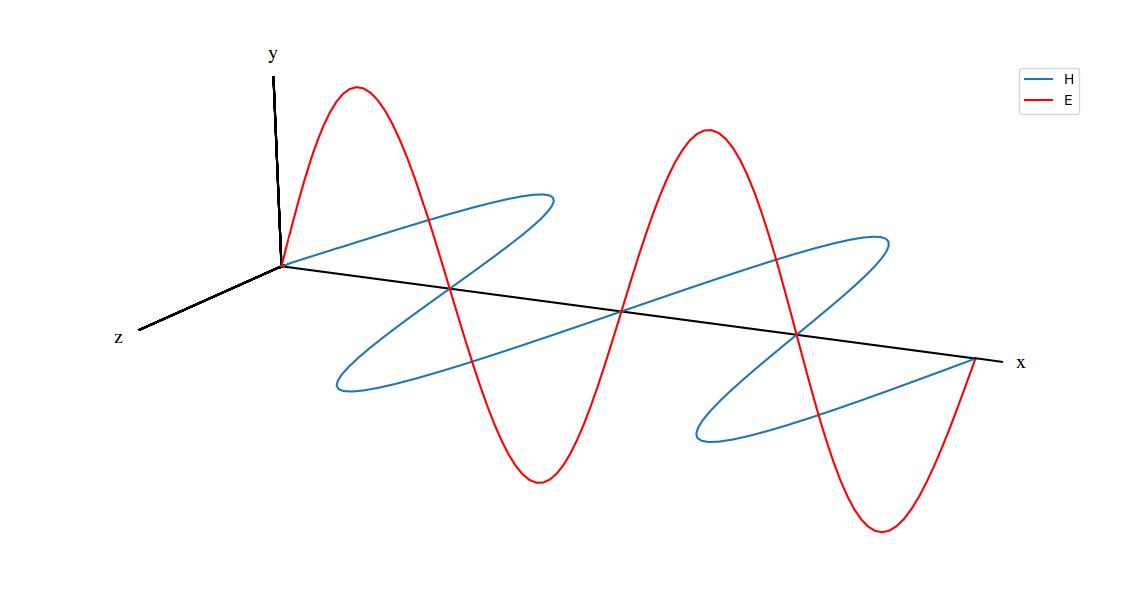
\includegraphics[scale=0.3]
			{images/fig2.png}
	\end{center}
	\centering
	\fautor
\end{figure}

\subsection{Light Wave Properties}

The light waves can be represented by a ray, i.e. a single oriented line which shows the direction of propagation; several waves that propagate in nearly the same direction can be named as a beam \cite{halliday2013fundamentals}. These two models of the real light are important and useful representations within the boundaries of visible light, and allow easier explanations of light properties.

Rays or beams of light may come from a picometric scale source (due to nuclear processes) or from a relatively larger scale, e.g. the fluorescent and incandescent light bulbs, which are sources of electric light. Eventually, light reaches surfaces during its propagation, and this is the event that allows the human vision feature; when it occurs, there are three prominent phenomena to consider: reflection, refraction and diffraction. The incident ray of light suffers a split procedure when it reaches a frontier between two homogeneous media. One of the resulting rays propagates in the initial medium and the other one propagates inside the other medium; the first phenomenon is denominated \emph{reflection} and the second, \emph{refraction} \cite{born1999principles}.

The speed of light depends on the medium in which it propagates. The \emph{refractive index} is a number that quantifies the speed of light in a particular medium in relation to the speed of light a vacuum, and can be described by

\begin{equation}
    \label{eqn:refractive_index}
       n = \frac{c}{v}
\end{equation}

\noindent where $\mathit{c}$ is the speed of light in vacuum and $\mathit{v}$ is the speed of light in the medium. According to \citeonline{halliday2013fundamentals}, the reflection law states that the resulting ray propagates within the incidence plane and that the angle of reflection $\mathit{\theta^{'}_{1}}$ equals the $\mathit{\theta_{1}}$ angle of incidence; comparably, the refraction law states the same about the incidence plane and relates the incidence $\mathit{\theta_{1}}$ and refraction $\mathit{\theta_{2}}$ angles by Snell's law, given by

\begin{equation}
    \label{eqn:snells_law}
       n_{2}\sin{\theta_{2}} = n_{1}\sin{\theta_{1}}
\end{equation}

\noindent where $\mathit{n_{1}}$ and $\mathit{n_{2}}$ are the refractive indices of the media. This framework consists of an approximation and may be considered ideal for didactic purposes. The process that happens in the real situations may involve non-homogeneous media, opaque or translucent media (which blocks the propagation of light or randomly changes the direction of the rays, respectively), and those concepts are relevant to the imaging procedures, e.g. microscopy. Figure \ref{fig:beam_split} depicts the real-world phenomenon and its ideal representation.

\begin{figure}[htb]
	\centering
	\caption{\label{fig:beam_split} 
	    (a) Example of a beam of light that reflects and refracts when falling onto a frontier between air and water. (b) Representation of the process in terms of rays.}
	\begin{center}
	    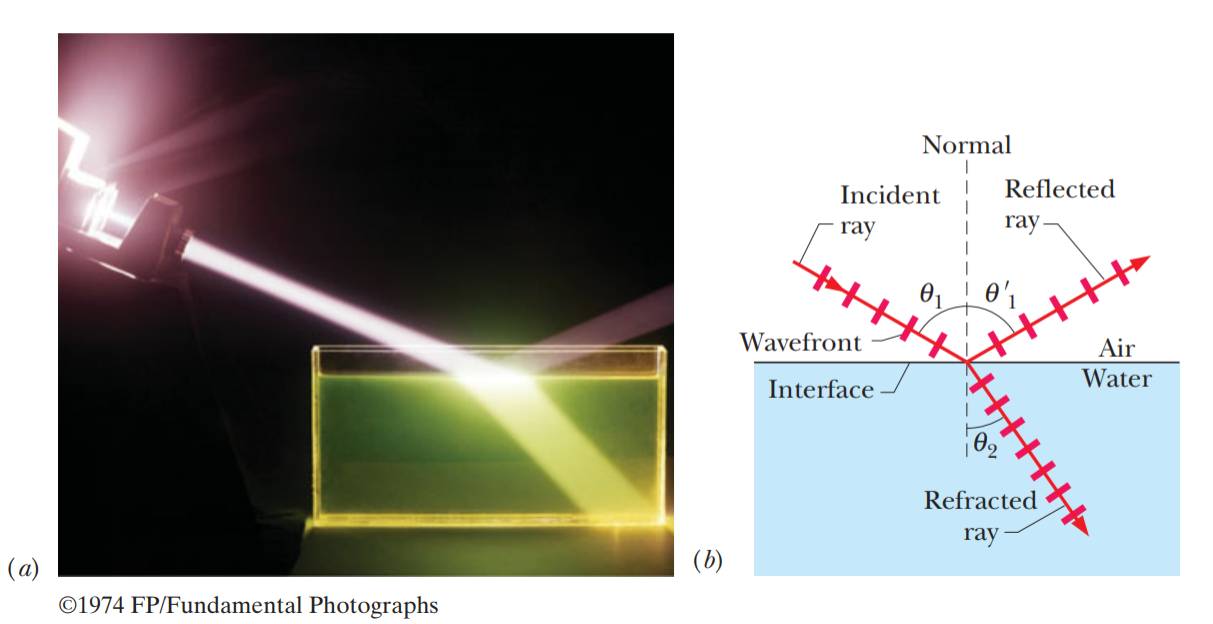
\includegraphics[scale=0.3]{images/fig3.png}
	\end{center}
	\centering
    \fdireta{halliday2013fundamentals}
\end{figure}

The wave theory of light also contains another important property for the real processes: the \emph{diffraction}, a phenomenon that was discovered by Francesco Maria Grimaldi (1618-1663) and consists of the distortion in a wavefront which focuses on obstacles such as apertures on an object, spheres, disks, or anything with similar dimension to the wavelength of the focusing light \cite{zilio2009optica}. The wavefront deviates and scatters after propagating through the obstacle and transforms itself into circular or spherical waves; this is a relevant property that distinguishes a wave from a particle, since the latter would either propagate without any change in its trajectory or would be blocked by the obstacle \cite{tipler2007physics}. When a beam of light reaches an opaque object, the waves suffer changes in their direction of propagation, which can be predicted by the fact that all the points in each wavefront (points of identical phase on waves) generate a new wave, as stated by Huygens \cite{fowles1989introduction}. The figure \ref{fig:diffraction} illustrates the diffraction phenomenon with an arbitrary obstacle and a small source of waves.

\begin{figure}[htb]
	\centering
	\caption{\label{fig:diffraction} Scheme of diffraction of a wavefront.}
	\begin{center}
	    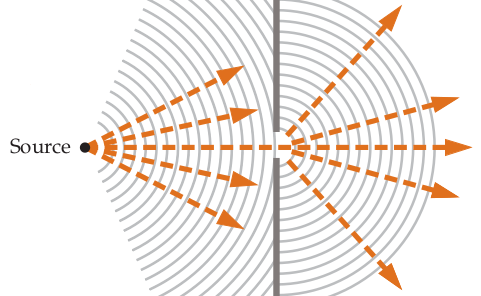
\includegraphics[scale=0.5]{images/diffraction.png}
	\end{center}
	\centering
    \fdireta{tipler2007physics}
\end{figure}

\subsection{Imaging Properties of Optical Systems}

Within the scope of this work, the main reason for introducing the concepts of optics is the imaging devices - the microscope, in particular. The structure of the apparatus will be described in Section \ref{sec:light_microscopy}. Moreover, a substantially large amount of devices rely on optical lenses for imaging, with properties such as depth of field and depth of focus.

As stated by \citeonline{halliday2013fundamentals}, \emph{lenses} are objects consisting of a transparent material, with a certain refractive index, that are made of two spherical surfaces on which light propagates and suffers refraction. They are used in optical systems due to their capacity to create images as long as their refractive index is not equal to that of the medium. Still, in agreement with \citeonline{halliday2013fundamentals}, some concepts related to lenses are important in our context and will be shown below. Figure \ref{fig:spherical_lens} denotes an illustration of an arbitrary spherical lens, and the following list depicts the principal elements from geometric optics that relates to lenses and its consequent imaging properties:

\begin{itemize}
    \item \emph{Radius of Curvature}: the distance between the center of the sphere and a refracting surface, named $\mathit{r_{1}}$ and $\mathit{r_{2}}$ on Figure \ref{fig:spherical_lens};
    
    \item \emph{Center of Curvature}: since the lenses are made by a union of two sections of a sphere-shaped object (which have a center), there are two Centers of Curvature for each lens, denoted by $\mathit{C_{1}}$ and $\mathit{C_{2}}$ on Figure \ref{fig:spherical_lens};
    
    \item \emph{Central Axis}: a line that represents the infinite number of radii of the sphere, which contain the center and the focal point;
    
    \item \emph{Focal Point}: also called \emph{focus}, a point within the central axis, where the image of the object is formed due to the convergence of the light rays from the object, and shown on Figure \ref{fig:spherical_lens} as $\mathit{F_{1}}$ and $\mathit{F_{2}}$;
    
    \item \emph{Focal Length}: presented as $\mathit{f}$ on Figure \ref{fig:spherical_lens}, it stands for the distance between the center of the sphere and the focal point;
    
    \item \emph{Object}: either a point or a surface on space that emits (or reflects) light and can be interpreted as a source;
    
    \item \emph{Image}: in this context, it is a representation of an object, formed by the action of lenses.
    
    \item \emph{Magnification}: a number that describes how larger or smaller the image will be in comparison to the object; mathematically, the ratio of the image distance to the object distance, both relative to the lens.
    
\end{itemize}

\begin{figure}[htb]
	\centering
	\caption{\label{fig:spherical_lens}Arbitrary scheme of the optical properties of a spherical lens.}
	\begin{center}
	    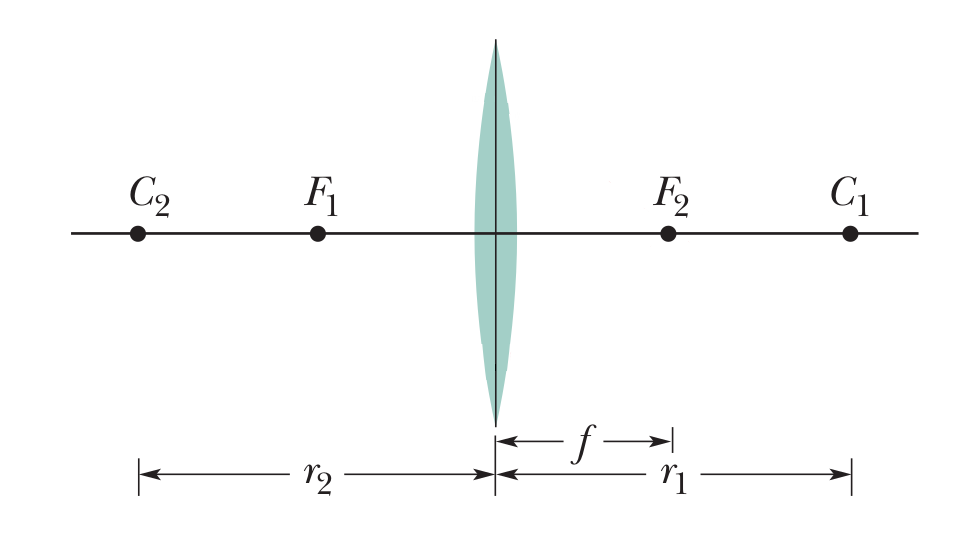
\includegraphics[scale=0.4]{images/fig4.png}
	\end{center}
	\centering
    \fadaptada{halliday2013fundamentals}
\end{figure}

A single lens or a set of lenses (most of the optical systems are more complicated than a single lens) have the \emph{depth of field} and the \emph{depth of focus} properties. Although the terms appear to be similar, the former relates to objects and the latter, to images \cite{davidson2002optical}. For every system, there is a focal plane in which the formed images will be sharp. Depth of Field is the tolerance for the object focal plane that may produce sharp images, while Depth of Focus dictates the same tolerance for the image focal plane. In other words, depth of field is the zone in the real world that would yield an acceptably sharp image and depth of focus is the same idea for the imaging sensors or for plotting the image.

{\color{red} Grammarly}
\section{Light microscopy}
\label{sec:light_microscopy}

The type of microscope discussed and used in this work is the light microscope; there are several techniques and approaches for employing optical lenses in order to obtain magnified images, but they are outside the bounds of this research. The compound light microscope is a device designed to generate magnified images from objects with the aid of visible light, and consists of two lenses: the \emph{objective} (closer to the object) and the \emph{ocular} (closer to the observer) \cite{murphy2012fundamentals}. This section presents some concepts and principles from the field.

\subsection{General Structure}

As reported by \citeonline{bell2009introduction}, the basic structure of a microscope consists of objective lenses, eyepieces, condensers, the stage and the light source, which are graphically described by Figure \ref{fig:compound_microscope} and explained as follows:

\begin{itemize}
    \item \emph{Objective Lenses}: a set of multiple lenses merged inside a tubular structure (barrel), which are designed for capturing light rays from the specimen or object and are built for minimizing the series of optical unwanted phenomena in imaging;

    \item \emph{Eyepieces}: lenses where the observer may look through, also inside a tubular structure, but with lower magnification in comparison to the objective;
    
    \item \emph{Condensers}: a collector of light from the light source, which sends the focus the rays on the object;
    
    \item \emph{Stage}: the support for the object; which may have height and positional adjustments in some devices;
    
    \item \emph{Light Source}: the main source of light, usually a lamp.
\end{itemize}

\begin{figure}[H]
	\centering
	\caption{\label{fig:compound_microscope}Graphic representation of the basic compound light microscope structure.}
	\begin{center}
	    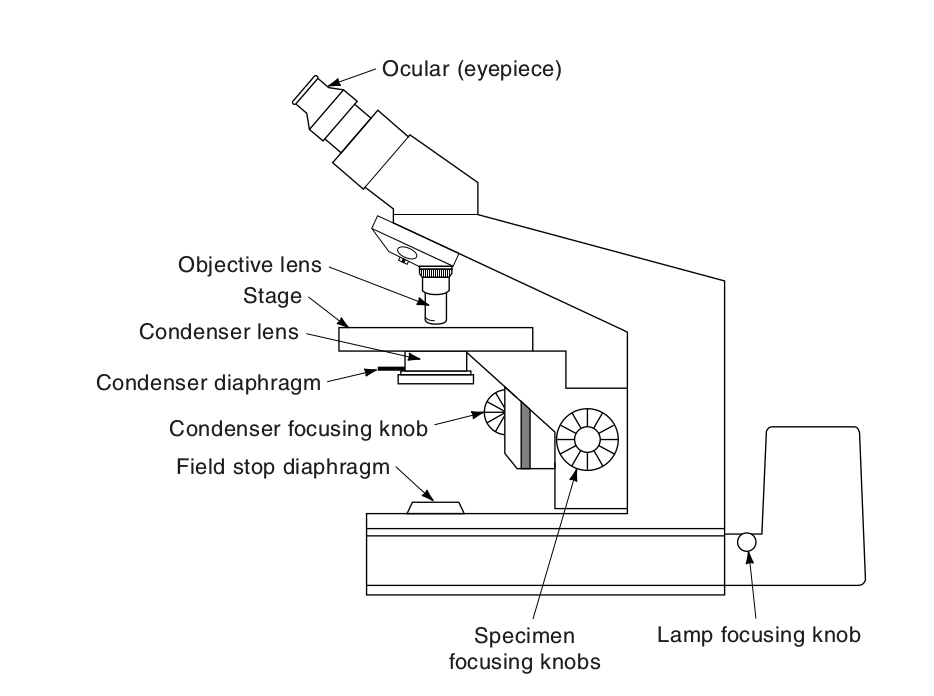
\includegraphics[scale=0.4]{images/fig5.png}
	\end{center}
	\centering
    \fdireta{bell2009introduction}
\end{figure}

Considering the fact that light is some sort of radiation, there are several different ways to achieve imaging in microscopes; it can be made by light, polarized light, lasers, X-rays, among others. There are also advanced techniques such as confocal microscopy, which is capable of imaging a very small area of the object, with all the light rays focused on it \cite{rochow1994introduction}. It all depends on the purpose of microscopy within the proposed task.

\subsection{Stereo Compound Microscope}


One of the versions of compound microscopes is the stereo microscope. It consists of a fusion of two compound microscopes in a convergent optical system, and may have two different objectives and eyepieces or only one objective and two eyepieces \cite{schreier2004advances}. The former is named \emph{binobjective-binocular} (Greenough) and the latter is named \emph{monobjective-binocular}, also named \sigla{CMO}{Common Main Objective Stereo Microscope}. One of the advantages of CMO microscopes is the higher depth of field, which allows the user to view and investigate biological specimens, relatively small materials and any kind of non-smooth surfaces. Furthermore, it is possible to view and acquire images on three dimensions \cite{rochow1994introduction}. The structure of both types of stereo compound microscopes are denoted by Figure \ref{fig:stereo_compound_microscope}

\begin{figure}[H]
	\centering
	\caption{\label{fig:stereo_compound_microscope}Graphic representation of the basic stereo compound light microscope structure, (a) for the Greenough type and (b) for the CMO.}
	\begin{center}
	    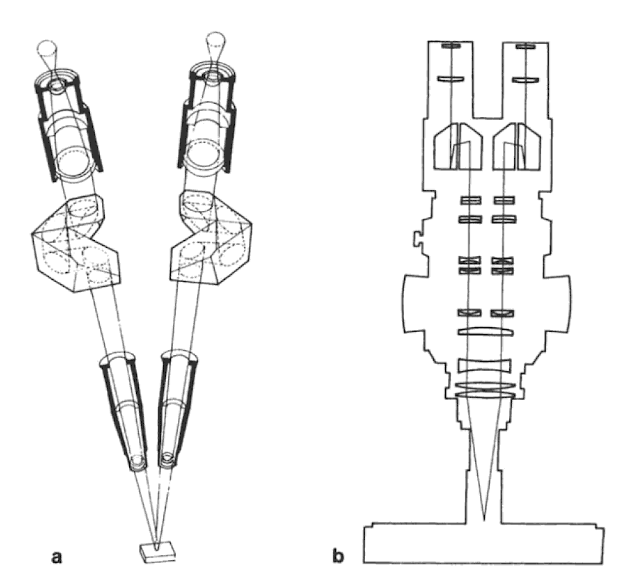
\includegraphics[scale=0.4]{images/fig6.png}
	\end{center}
	\centering
    \fdireta{rochow1994introduction}
\end{figure}